\hypertarget{ch:probability}{%
  \chapter{Intuition, Paradoxes, and Probability}
  \label{ch:probability}}

\chapterartfile{images/Black_Dice_PNG_Clip_Art-2653.png}
\hypertarget{Rintro}{The world is random and probability is a tool to quantify
  the randomness. With random events, our intuition may give us high confidence
  on a wrong conclusion. For example, knowing that A is larger than B and B is
  larger than C, can we say A is always larger than C? Not really for random
  events.}

\hypertarget{probability}{%
\section{Probability}\label{probability}}

We will go through examples to see how probability helps
interpret phenomena in real life and how probability may counter
intuition. We begin by introducing some concepts:
\begin{itemize}
\item Experiment: a situations in which the outcome occur randomly, e.g.,
  flipping a coin, rolling a dice, and picking a card.
\item Sample Space: the set of all possible outcomes in an experiment, e.g.,
  \{head, tail\}, \{1, 2, ..., 6\}, and \{all card faces\}.
\item Event: a subset of the sample space is called an event; an event
  occur if the outcome from an experiment belong to the event. For example, if
  you roll a dice, and you are interested in the result of having an even number,
  then the event is $E$=\{2, 4, 6\}.
\end{itemize}

The relationship between a sample space and an event can be illustrated using a
Venn diagram such as Figure~\Ref{fig:probability-event} for rolling a dice. The
sample space labeled as $S$ is represented as the rectangle that contains all the
six possible outcomes. The event $E$ of having an even number is represented
as the circle that contains the even numbers.

\begin{figure}[htbp]
\centering
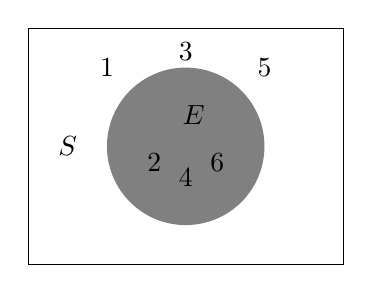
\begin{tikzpicture}
  \draw (-2, 1.5) rectangle (2, -1.5);
  \fill[color=gray] (0, 0) circle (1);
  \draw (-1.5, 0) node{$S$};
  \draw (-1, 1) node{1} (0, 1.2) node{3} (1, 1) node{5};
  \draw (0.1, 0.4) node{$E$};
  \draw (-0.4, -0.2) node{2} (0, -0.4) node{4} (0.4, -0.2) node{6};
\end{tikzpicture}
\caption{Sample space and event illustrated with Venn diagram}
\label{fig:probability-event}
\end{figure}

\emph{Probability} is a measure on how likely an event occurs. If we assume that the
possible outcomes in an experiment % is countable and they
have equal chance to occur, then the probability of event $E$ is
  \begin{equation}
    P(E) =\frac{\text{size of } E}{\text{size of } S}.
  \end{equation}
  % where $n$ is the number of elements in $E$ and $N$ is the
  % number of elements in the sample space.  Note that this formula
  % holds only if all the outcomes are equally likely.

% \hypertarget{example-elevator-waiting-time}{%
%   \section{Elevator waiting
%     time}\label{example-elevator-waiting-time}}
\begin{example}[Elevator waiting time]
  Mr. Smith works on the 13th floor of a 15 floor building. The only elevator
  moves continuously through floors 1, 2, . . . 14, 15, 14, . . . 2, 1, 2,
  . . . , except that it stops on a floor on which the button has been
  pressed. Assume that time spent loading and unloading passengers is very small
  compared to the travelling time.  Mr.~Smith complains that at 5pm, when he
  wants to go home, the elevator almost always goes up when it stops on his
  floor. What is the explanation?
\end{example}

When Mr.~Smith gets to the elevator, it may be below the 13th floor or above
it. The elevator will goes up if it is below the 13th floor and it will goes
down if it is above the 13th floor. There are 12 floors below the 13th floor and
2 floors above it, so the probability that the elevator is below the 13th floor
is $12/14\approx0.86>0.5$. Thus no matter when Mr. Smith wants to go home, it is
more likely that the elevator is going up.

We can simulate this situation:

\showCode{R}{Code/probability-elevator.R}
\runR{Code/probability-elevator.R}{elevator}{}
Running the above code gives:
\includeOutput{elevator}
%%%%%%%%%%%%%%%%%%%%%%%%%%%%%%%%%%%%
%\input{Rnw/probability-elevator}

Probabilities for random may counter intuition and they may not have usual
ordering. We discus two examples in the following subsections.

\hypertarget{Intransitive-Dice}{%
  \subsection{Intransitive Dice}\label{Intransitive-Dice}}

We know that in general if $A>B$ and $B>C$ then $A>C$. However, this may not be
the case in the word of probability.

\begin{example}[Intransitive Dice]
% Consider three dice with different sides numbers:
\begin{itemize}
\item Die A has sides 2, 2, 4, 4, 9, 9.
\item Die B has sides 1, 1, 6, 6, 8, 8.
\item Die C has sides 3, 3, 5, 5, 7, 7.
\end{itemize}
\end{example}

To play a game using dice A and B, you can chose which die to roll and your
opponent rolls the other. The one who tolls a larger number wins. Which die do
you want to choose?

Let's table the possible results to see the better die.
\begin{center}
  \begin{tabular}{cc|ccc}\hline
    &   & \multicolumn{3}{c}{B} \\
    % \cline{3-5}
    &   & 1                & 6                & 8                \\ \hline
    \multirow{3}{*}{A}
    & 2 & \color{red}$A>B$ & $A<B$            & $A<B$            \\
    & 4 & \color{red}$A>B$ & $A<B$            & $A<B$            \\
    & 9 & \color{red}$A>B$ & \color{red}$A>B$ & \color{red}$A>B$ \\\hline
  \end{tabular}
\end{center}

Since die A wins five out of the nine possible results and all possible results
occur with equal probability, we know that die A has a higher winning
probability ($\frac{5}{9}$) than die B. We should choose die A over die B.

Now consider dice B and C.
\begin{center}
  \begin{tabular}{cc|ccc}\hline
    &   & \multicolumn{3}{c}{B} \\
    % \cline{3-5}
    &   & 1                & 6                & 8                \\ \hline
    \multirow{3}{*}{C}
    & 3 & \color{red}$C>B$ & $C<B$            & $C<B$            \\
    & 5 & \color{red}$C>B$ & $C<B$            & $C<B$            \\
    & 7 & \color{red}$C>B$ & \color{red}$C>B$ & $C<B$ \\\hline
  \end{tabular}
\end{center}

We see that die B has a higher winning probability ($\frac{5}{9}$) than die C,
so we should choose die B over die C.

Since we should choose die A over die B, and choose die B over die C, does this
mean that we should choose die A over die C if these two dice are to be
selected. Surprisingly, the answer is NO. Here is the table of the possible
results.
\begin{center}
  \begin{tabular}{cc|ccc}\hline
    &   & \multicolumn{3}{c}{C} \\
    % \cline{3-5}
    &   & 3                & 5                & 7                \\ \hline
    \multirow{3}{*}{A}
    & 2 & $A<C$            & $A<C$            & $A<C$            \\
    & 4 & \color{red}$A>C$ & $A<C$            & $A<C$            \\
    & 9 & \color{red}$A>C$ & \color{red}$A>C$ & \color{red}$A>C$ \\\hline
  \end{tabular}
\end{center}
We should choose die C over die A!

Here is an experiment to simulate the intransitive dice.

% \showCode{python}{Code/probability-IntransitiveDice.py}
% Running this code gives the following:
% \runPython{Code/probability-IntransitiveDice.py}{IntransitiveDice}{}
% \includeOutput{IntransitiveDice}
\showCode{R}{Code/probability-IntransitiveDice.R}
Running this code gives the following:
\runR{Code/probability-IntransitiveDice.R}{IntransitiveDice}{}
\includeOutput{IntransitiveDice}

%%%%%%%%%%%%%%%%%%%%%%%%%%%%%%%%%%%%
%\input{Rnw/probability-IntransitiveDice}

\hypertarget{birthday-problem}{%
  \subsection{Birthday Problem}\label{birthday-problem}}

\begin{example}[Birthday Problem]
Suppose that a room contains 23 people. What is the probability that
at least two of them have a common birthday? Assuming that each year has 365
days, this probability seems very small, but it is actually about
0.5. What is the probability that some one in that room has the same
birthday as yours? This probability is quite small
($\approx0.061$). In order to have the probability that someone's
birthday is the same as yours to be 0.5, we need 253 random selected people to
be in that room.
\end{example}

Let's use simulation to verify the aforementioned numbers.

\showCode{R}{Code/probability-birthday.R}
\runR{Code/probability-birthday.R}{birthday}{}
Running the above code gives:
% \includeOutput{birthday}
If there are 23 people in the room, the probability that some people
share the same birthday is \inlnR{```cat(prob.p23[1])```} and the probability
that some people's birthday is the same as yours is
\inlnR{```cat(prob.p23[2])```}. If there are 253 people in the room, the two
probabilities are \inlnR{```cat(prob.p253[1])```} and \inlnR{```cat(prob.p253[2])```}, respectively. 
%%%%%%%%%%%%%%%%%%%%%%%%%%%%%%%%%%%%
%\input{Rnw/probability-birthday}

% \begin{equation*}
%   P(A)=1-P(A^c)=1-\frac{P_{365,n}}{365^n}=1-\frac{365\times364\times\cdots
%                  \times(365 - n + 1)}{365^n}
% \end{equation*}
% Some numbers:\\
% \begin{tabular}{lrrrrrr}\hline
%   $n$ & 4 & 16 & 23 & 32 & 40 & 56 \\
%   \hline
%   $P(A)$ & .016 & .284 & .507 & .753 & .891 & .988 \\\hline
% \end{tabular}
% \begin{equation*}
%   P(A)=1-P(A^c)=1-\frac{364^n}{365^n}
% \end{equation*}

\hypertarget{conditional}{%
\section{Conditional Probability}\label{conditional}}

Additional knowledge may affect the outcome of an experiment and change
the probability of an event. This is the \emph{conditional probability}. For example, when there are two events $A$ and $B$
in consideration, knowing that $A$ has occurred may change the probability for
$B$ to occur, and it is called the probability of event $B$ given event $A$. In
Figure~\Ref{fig:probability-conditional}, the probability of event $B$ without
known the occurrence of event $A$ is
\begin{equation}
  P(B)=\frac{\text{size of } B}{\text{size of } S}
  =\frac{\text{size of (2) + (3)}}{\text{size of } S}.
\end{equation}
This is an \emph{unconditional probability}. If we know that $A$ has occurred,
then the area of $A$ becomes the sample space and the outcome much be in the
area of (2) for $B$ to occur. Thus the \emph{conditional probability} of $B$
given $A$ is
\begin{equation}
  P(B\mid A)=\frac{\text{size of (2)}}{\text{size of } A}
  =\frac{\text{size of (2)}}{\text{size of (1) + (2)}}.
\end{equation}

\begin{figure}[H]
\centering
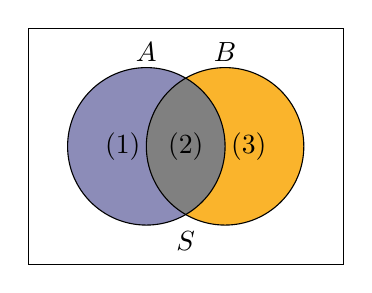
\begin{tikzpicture}
\draw (-2, 1.5) rectangle (2, -1.5);
\fill[color=MidnightBlue!50] (-0.5, 0) circle (1);
\fill[color=Dandelion] ( 0.5, 0) circle (1);
\begin{scope}
  \clip (-0.5,0) circle(1);
  \clip (0.5,0) circle(1);
  \fill[gray](0,0) circle(1);
\end{scope}
\draw (-0.5, 0) circle (1);
\draw ( 0.5, 0) circle (1);
\draw ( 0, -1.2) node{ $S$};
\draw (-0.5, 1.2) node{ $A$};
\draw ( 0.5, 1.2) node{ $B$};
\draw (-0.8, 0) node{ $(1)$};
\draw (   0, 0) node{ $(2)$};
\draw ( 0.8, 0) node{ $(3)$};
\end{tikzpicture}
\caption{Probabilities with two events}
\label{fig:probability-conditional}
\end{figure}

% \hypertarget{Two-Child}{%
%   \section{Two Children}\label{Two-Child}}

\begin{example}[Two Children]
Consider the following two problems:
\begin{enumerate}
\item Mr. Jones has two children. The older child is a girl. What is the
  probability that both children are girls?
\item Mr. Smith has two children. At least one of them is a girl. What is the
  probability that both children are girls?
\end{enumerate}
\end{example}
Here are the possibilities of \{older child, younger child\}: \{Boy, Boy\},
\{Boy, Girl\}, \{Girl, Boy\}, \{Girl,Girl\}, with equal probabilities to occur.

For the first question: two elements satisfy the situation (the sample space for
the given situation) -- \{Girl, Boy\}, \{Girl,Girl\}; one element corresponds to
the event of two girls. Thus the
probability of two girls is $\frac{1}{2}$. This question can also be solved this
way: Since the older child is a girl, the probability of two girls is the
probability that the younger child is a girl which is $\frac{1}{2}$.

For the second question, three elements satisfy the situation (the sample space
for the given situation): \{Boy, Girl\}, \{Girl, Boy\}, \{Girl,Girl\}. Thus the
probability is $\frac{1}{3}$.

If we simulate many families, we can find the numerical answer quite accurately.

\showCode{R}{Code/probability-TwoChildren.R}
\runR{Code/probability-TwoChildren.R}{TwoChildren}{}
Running the above code gives:
\includeOutput{TwoChildren}
%%%%%%%%%%%%%%%%%%%%%%%%%%%%%%%%%%%%
%\input{Rnw/probability-TwoChildren}


% \hypertarget{Fair-Division}{%
%   \section{Fair Division}\label{Fair-Division}}

\begin{example}[Fair Division]
Tom and Jerry, each put 30 dollar in a jackpot to start a game. Suppose that
they have equal chance to win and the one who wins three times takes all the 60
dollars. Now, Tom has won twice and Jerry has won once, but then something
happens and the game must be stopped. How should they split the 60 dollars
according their probabilities of winning if the game was finished?
\end{example}

It seems Tom has won twice and Jerry has won once so the 60 dollars should be
split as $40:20$. However, these are not proportional to their probabilities of
winning. They need at most another two games to know the final winner. Here are
the four possible results of the two games: \{Tom, Tom\}, \{Tom, Jerry\},
\{Jerry, Tom\}, \{Jerry, Jerry\}. The probabilities that Tom and Jerry would be
the final winner are $\frac{3}{4}$ and $\frac{1}{4}$, respectively, so the fair
division should be $45:15$.

Let's use simulation to solve this problem.

\showCode{R}{Code/probability-FairDivision.R}
\runR{Code/probability-FairDivision.R}{FairDivision}{}
Running the above code gives:
\includeOutput{FairDivision}
%%%%%%%%%%%%%%%%%%%%%%%%%%%%%%%%%%%%
%\input{Rnw/probability-FairDivision}


% \hypertarget{Henry-Choice}{%
%   \section{Henry's Choice}\label{Henry-Choice}}

\begin{example}[Henry's Choice]
Henry has been caught stealing cattle, and is brought into town for justice. The
judge is his ex-wife Gretchen, who wants to show him some sympathy, but the law
clearly calls for two shots to be taken at Henry from close range. To make
things a little better for Henry, Gretchen tells him she will place two bullets
into a six-chambered revolver in successive order. She will spin the chamber,
close it, and take one shot. If Henry is still alive, she will then either take
another shot, or spin the chamber again before shooting.

Henry is a bit incredulous that his own ex-wife would carry out the punishment,
and a bit sad that she was always such a rule follower. He steels himself as
Gretchen loads the chambers, spins the revolver, and pulls the trigger. Whew! It
was blank. Then Gretchen asks, ``Do you want me to pull the trigger again, or
should I spin the chamber a second time before pulling the trigger?'' What
should Henry choose?
\end{example}

We know that the first chamber Gretchen fired was one of the four empty
chambers. Since the bullets were placed in consecutive order, one of the empty
chambers is followed by a bullet, and the other three empty chambers are
followed by another empty chamber. So if Henry has Gretchen pull the trigger
again, the probability that a bullet will be fired is 1/4.

If Gretchen spins the chamber again, the probability that she shoots Henry would
be 2/6, or 1/3, since there are two possible bullets that would be in firing
position out of the six possible chambers that would be in position.

\showCode{R}{Code/probability-HenryChoice.R}
\runR{Code/probability-HenryChoice.R}{HenryChoice}{}
Running the above code gives:
\includeOutput{HenryChoice}
%%%%%%%%%%%%%%%%%%%%%%%%%%%%%%%%%%%%
%\input{Rnw/probability-HenryChoice}


\hypertarget{further}{%
\section{Further Examples}\label{further}}

\hypertarget{Bertrand-Box}{%
\subsection{Bertrand's Box}\label{Bertrand-Box}}

\begin{example}[Bertrand's Box]
Bertrand's box paradox was first posed by Joseph Bertrand 1889. Here is the
question: There are three boxes, one contains two gold coins, one contains two
silver coins, and one contains a gold coin and a silver coin.
A box is selected at random and a coin is taken from that box at random. If the
coin is a gold coin, what is the probability that the other coin in that box is
also a gold coin.
\end{example}

This problem is about conditional probability. It is easy to find the
probability of getting a certain box, and it is easy to find the probability of
getting a gold coin if we know the box, as shown in
Figure~\ref{fig:probability-flow}. However, it is non-trivial to find the
difficulty of getting a certain box when we know the final coin. We see the six
possible outcomes in Figure~\ref{fig:probability-flow} are equally likely to
occur. Two outcomes of a gold coin are through the path of the box with two gold
coins and one outcome of a gold coin is through the path of the box with a gold
coin and a silver coin. Thus the answer to this problem is $\frac{2}{3}$.

\begin{figure}[H]
\centering
\resizebox{0.6\columnwidth}{!}{%
\begin{tikzpicture}[%scale=0.5,
  edge from parent/.style={draw,-latex},
    boxes/.style={star, draw=none, fill=red, drop shadow, text centered, anchor=north},
    state/.style={draw=none, fill=red, circle, drop shadow, text centered, anchor=north},
    leaf/.style={draw=none, fill=orange, ellipse, text centered, anchor=north},
    leafs/.style={draw=none, fill=gray, ellipse, text centered, anchor=north},
    level distance=0.9cm, growth parent anchor=south
]
\node [boxes] {Boxes} [->] [sibling distance=4cm]
child{ [sibling distance=2cm]
  node [state] {Gold, Gold}
  child{node [leaf] {Gold}
    edge from parent{node[left]{$\frac{1}{2}$}}
  }
  child{node [leaf] {Gold}
    edge from parent{node[right]{$\frac{1}{2}$}}
  }
  edge from parent{node[above right]{$\frac{1}{3}$}}
}
child{ [sibling distance=2cm]
  node [state] {Gold, Silver}
  child{node [leaf] {Gold}
    edge from parent{node[left]{$\frac{1}{2}$}}
  }
  child{node [leafs] {Silver}
    edge from parent{node[right]{$\frac{1}{2}$}}
  }
  edge from parent{node[right]{$\frac{1}{3}$}}
}
child{ [sibling distance=2cm]
  node [state] {Silver, Silver}
  child{node [leafs] {Silver}
    edge from parent{node[left]{$\frac{1}{2}$}}
  }
  child{node [leafs] {Silver}
    edge from parent{node[right]{$\frac{1}{2}$}}
  }
  edge from parent{node[above right]{$\frac{1}{3}$}}
};
\end{tikzpicture}
}
\caption{Probability flow for Bertrand's Box}
\label{fig:probability-flow}
\end{figure}

This problem can also be solved using the Bayesian formula. It says 
\begin{align}
  P(B\mid A) = \frac{P(A\mid B)P(B)}{P(A)},
\end{align}
where the conditional probability $P(B\mid A)$ is difficult to find but the
conditional probability $P(A\mid B)$ as well as the unconditional probabilities
are easy to find. If $A$ be the event of getting a gold coin and $B$ be the
event of getting a box with two gold coins, then $P(A)=\frac{1}{2}$,
$P(B)=\frac{1}{3}$, and $P(A|B)=1$. Now the probability of a box with two gold
coins given a final gold coin is 
\begin{align}
  % P(GG\mid G) = \frac{P(G\mid GG)P(GG)}{P(G)}
  P(B\mid A) = \frac{P(A\mid B)P(B)}{P(A)}
  = \frac{1\times\frac{1}{3}}{\frac{1}{2}}
  =\frac{2}{3}.
\end{align}

Both of the aforementioned two approaches give us the correct answer. However,
we don't have to go through the counting or reasoning. If we can simulate the
game, we can find the result pretty accurately. The following code simulate the 
game and approximate the probability numerically.

\showCode{R}{Code/probability-BertrandBox.R}
\runR{Code/probability-BertrandBox.R}{BertrandBox}{}
Running the above code gives:
\includeOutput{BertrandBox}

\hypertarget{Monty-Hall-problem}{%
\subsection{Monty Hall problem}\label{Monty-Hall-problem}}

\begin{example}[Monty Hall Problem]
Suppose you're on a game show, and you're given the choice of three doors:
Behind one door is a car; behind the others, goats. You pick a door, say No. 1,
and the host, who knows what's behind the doors, opens another door, say No. 3,
which has a goat. He then says to you, ``Do you want to pick door No. 2?'' Is it
to your advantage to switch your choice?
\end{example}

This famous example has confused many smart people. It is also about conditional
probability and can be solved by using the Bayesian formula. However, setting up
the conditional and unconditional probabilities for this problem is
complicated. Some people did not believe the result answer until they see some
simulations. The following code provide a simulation based on \code{n=1000}
repetitions.   

\showCode{R}{Code/probability-MontyHall.R}
\runR{Code/probability-MontyHall.R}{MontyHall}[run]
Running the above code gives:
\includeOutput{MontyHall}

We see that the probability of winning a car is much higher than 0.5 if one
chooses to switch. 

\hypertarget{simpsons-paradox}{%
\subsection{Simpson's Paradox}\label{simpsons-paradox}}

It is a phenomenon in which a trend appears in several different
groups of data but disappears or reverses when these groups are
combined. 

% \jy{we may define an example environment and a comment/discussion environment}
% \textbf{An urn example}:
\begin{example}[Combined urns]
A black urn contains 5 red and 6 green balls,
and a white urn contains 3 red and 4 green balls. You are allowed to
choose an urn and then choose a ball at random from the urn. If you
choose a red ball, you get a prize. Which urn should you choose to
draw from?
\begin{itemize}
\item If you draw from the black urn, the probability of choosing a
  red ball is $5/11 = .455$.
\item If you choose to draw from the white urn, the probability of
  choosing a red ball is $3/7 = .429$.
\end{itemize}
You should choose to draw from the black urn.

Now consider another game in which a second black urn has 6 red and
3 green balls, and a second white urn has 9 red and 5 green balls.
\begin{itemize}
\item If you draw from the black urn, the probability of a red ball is
  $6/9 = .667$.
\item If you choose to draw from the white urn, the probability if
  $9/14 = .643$.
\end{itemize}
Again you should choose to draw from the black urn.

In the final game, the contents of the second black urn are added to
the first black urn, and the contents of the second white urn are
added to the first white urn. Again, you can choose which urn to draw
from. Which should you choose?

Intuition says choose the black urn, but let's calculate the
probabilities.
\begin{itemize}
\item The black urn now contains 11 red and 9 green balls, so the
  probability of drawing a red ball from it is 11/20=0.55
\item The white urn now contains 12 red and 9 green balls, so the
  probability of drawing a red ball from it is 12/21= .571.
\end{itemize}
You should choose the white urn!
\end{example}

% \textbf{UC Berkeley gender bias:}
\begin{example}[UC Berkeley gender bias]
A famous example of Simpson's
paradox is a study of gender bias among graduate school admissions to
University of California, Berkeley. In 1973 UC Berkeley was sued for
sex-discrimination. Here are the overall numbers for the six largest
departments in fall admission of 1973.

\begin{table}[H]
\begin{center}
  \begin{tabular*}{\textwidth}{@{\extracolsep{\fill}}crrcrr}
    \toprule
    \multicolumn{3}{c}{Men} & \multicolumn{3}{c}{Women} \\
    \cmidrule(lr){1-3}\cmidrule(lr){4-6}
    Applicants & \multicolumn{2}{c}{Admitted} & Applicants
                                              & \multicolumn{2}{c}{Admitted} \\
    \midrule
    2691 & 1198 & ({\bf 44.5}\%) & 1835 & 557 & (30.4\%) \\
    \bottomrule
  \end{tabular*}
\end{center}
\end{table}

This table shows that men were more likely than women to be admitted,
and the difference was so significant. Let's see which departments
were mainly responsible for this gender bias. To do this we broke open
the data according to each departments.

\begin{table}[H]
\centering
\begin{tabular*}{\textwidth}{@{\extracolsep{\fill}} ccrrcrr}
  \toprule
  & \multicolumn{3}{c}{Men}  & \multicolumn{3}{c}{Women} \\
  \cmidrule(lr){2-4}\cmidrule(lr){5-7}
  Department & Applicants  & \multicolumn{2}{c}{Admitted} & Applicants
                           & \multicolumn{2}{c}{Admitted} \\
  \midrule
A & 825 & 512& (62\%) & 108 & 89 &(82\%)  \\ 
B & 560 & 353& (63\%) & 25  & 17 &(68\%)  \\
C & 325 & 120& (37\%) & 593 & 202& (34\%) \\
D & 417 & 138& (33\%) & 375 & 131& (35\%) \\
E & 191 & 53 & (28\%) & 393 & 94 &(24\%)  \\
F & 373 & 22 & (6\%) & 341 & 24 &(7\%)  \\
  \bottomrule
\end{tabular*}
\end{table}
% \jy{we need to set some style guidelines on code, floats, etc.}

Things get strange after we divide the data according different
departments. For the six departments, four of them accepted women more
than men.  To explain this, \cite{bickel1975sex} noticed that women
tended to apply to more competitive departments with low admission
rates even among qualified applicants, whereas men tended to apply to
less competitive departments with high admission rates among the
qualified applicants.
\end{example}

To use simulation to further illustrate this, we simulate a data set
with four groups in the following.

\showCode{R}{Code/probability-Simpson.R}[1][6]
\runR{Code/probability-Simpson.R}{Simpson}{}
% Running the above code gives:
% \includeOutput{Simpson}

We use the following code to first plot the whole data and then mark different
groups in different colors. 
\showCode{R}{Code/probability-Simpson.R}[8][9]


\begin{figure}[H]
\centering
\includegraphics[width=0.45\textwidth]{images/probability-Simpson-plots.pdf}
\includegraphics[width=0.45\textwidth,page=2]{images/probability-Simpson-plots.pdf}
\caption{Scatter plot of the whole data without (left) and with (right) group labeled.}
\label{fig:probability-simpson}
\end{figure}


The results are displayed in Figure~\ref{fig:probability-simpson}.
For the whole data $y$ has an increase pattern as $x$ increases, but for each
sub group $y$ has a decrease pattern as $x$ increases. 


% \hypertarget{prisoners-problem}

The technique of simulation is useful in finding answers in very complicated
problems. Consider the following example modified from
\cite{flajolet2009analytic}.

\begin{example}[100 Prisoners]
In a prison, there are 100 death row prisoners who are numbered from 1
to 100, and there is a room with 100 drawers labeled from 1 to
100. The director randomly puts one prisoner's number in each closed
drawer and offers a last chance. The prisoners enter the room, one
after another. Each prisoner may open and look into 50 drawers in any
order. The drawers are closed again afterwards. If, during this
search, every prisoner finds his number in one of the drawers, all
prisoners are pardoned. If some prisoner does not find his number, all
prisoners die. Before the first prisoner enters the room, the
prisoners may discuss strategy, but they cannot communicate once the
first prisoner enters the room.
\end{example}

The situation is hopeless if every prisoner selects fifty drawers at
random. The probability that a single prisoner finds his number is
0.5, so the probability that all prisoners find their numbers is
$0.5^{100} = 7.89\times10^{-31}\approx0$. However, a better strategy
% gives the prisoners more than 0.30 probability to survive
is given in \citep{stanley2013algebraic}, which is described below:
\begin{enumerate}
\item Each prisoner first opens the drawer with his own number.
\item If this drawer contains his number he is done and was
  successful.
\item Otherwise, the drawer contains the number of another prisoner
  and he next opens the drawer with this number.
\item The prisoner repeats steps 2 and 3 until he finds his own number
  or has opened 50 drawers.
\end{enumerate}

This strategy is better than randomly opening because it utilizes the
information from other prisoners. For example, different prisoners all start
from opening different drawers, while it is almost certain that some prisoners
start from opening the same drawer {\color{red} WHY: this may be an exercise
problem.}. The probability of survival with the this strategy is complicate to
derive analytically.

In the following, we define two functions to simulate the method of randomly
open 50 drawers and the better strategy, respectively.

\showCode{R}{Code/probability-100prisoners.R}
\runR{Code/probability-100prisoners.R}{100prisoners}[cache]
Running the above code gives:
\includeOutput{100prisoners}

We see that opening drawers randomly has a survival probability of almost zero
while the smarting strategy gives a survival probability close to 0.3.

%%% Local Variables:
%%% mode: latex
%%% TeX-command-extra-options: "-shell-escape"
%%% TeX-engine: xetex
%%% TeX-master: "../sidsmain.tex"
%%% End: